% % % % % % % % % % % % % % %
\documentclass[11pt]{article}
\usepackage[a4paper, portrait, margin=1in]{geometry}
% % % % % % % % % % % % % % %

\usepackage{amssymb}
\usepackage{xcolor}
\usepackage{fancyhdr}
\usepackage{mathtools}
\usepackage{amsthm}
\usepackage{verbatim}
\usepackage{hyperref}
\usepackage{footnotebackref}
\usepackage[labelfont=bf]{caption}
\usepackage{subcaption}
\usepackage{colortbl}
\usepackage{multirow}
\usepackage{hhline}
\usepackage{tikz}

\usetikzlibrary{arrows}

\pagestyle{fancy}
\fancyhf{}
\renewcommand{\headrulewidth}{0pt}
\renewcommand{\footrulewidth}{0pt}

\fancypagestyle{firstpagefooter}
{
\lfoot{Version: 25.11.2016}
\cfoot{}
\rfoot{\thepage}
}
\cfoot{\thepage}

\hypersetup
{
    colorlinks=true,
    linkcolor=blue,
    citecolor=blue,
    filecolor=blue,
    urlcolor=blue,
    linktoc=page            % Link only on page number
}

\newcommand\task[1]{{\color[HTML]{999999}\subsection{Task}#1}}
\renewcommand\task[1]{}

\definecolor{Gray}{gray}{0.85}
\DeclarePairedDelimiter{\ceil}{\lceil}{\rceil}
\renewcommand{\qedsymbol}{$\diamondsuit$}
\newtheorem{hyp}{Hypothesis}
\newtheorem{rem}{Remark}
\theoremstyle{definition}
%\newtheorem*{ana}{Analysis}
\newenvironment{ana}[1][\proofname]{\begin{proof}[Analysis]}{\end{proof}}
\newcommand\re[1]{{\color[HTML]{ee1111}#1}}
\newcommand\gr[1]{{\color[HTML]{11aa11}#1}}
\newcommand\bl[1]{{\color[HTML]{1111dd}#1}}

% Timestamps (DO NOT CHANGE!)
\newcommand\Tarr{t_{\mathrm{arr}}}
\newcommand\Tenq{t_{\mathrm{enq}}}
\newcommand\Tdeq{t_{\mathrm{deq}}}
\newcommand\Tsent{t_{\mathrm{sent}}}
\newcommand\Trecv{t_{\mathrm{recv}}}
\newcommand\Tleft{t_{\mathrm{left}}}
\newcommand\Ttot{T_{\mathrm{tot}}}
\newcommand\Tque{T_{\mathrm{que}}}
\newcommand\Tsrv{T_{\mathrm{srv}}}
\newcommand\Tpro{T_{\mathrm{pro}}}

% Macros.
\newcommand\df\doteq
\newcommand\E[1]{\mathbb E[#1]}
\newcommand\V[1]{\mathbb V[#1]}
%\renewcommand\E{\mathbb E}
%\renewcommand\V{\mathbb V}
\renewcommand\b[1]{{\bf{#1}}}
\newcommand\p{^\prime}
\renewcommand\t\texttt
\newcommand\md[2]{\left[#1\mathrm{\ mod\ }#2\right]}
\newcommand\td{{\color{red}\b{\textsf{[TODO]}}}}
\newcommand\tpssnd{03_maximum_throughput_16-11-11_21:56:33}
\newcommand\repl{04_replication_effect_16-11-20_13:16:14}
\newcommand\wh[1]{{\color[HTML]{FFFFFF}#1}}

\begin{document}

\title{Advanced Systems Lab (Fall'16) -- Third Milestone}

\author{Name: \emph{Fabio M. Banfi}\\Legi number: \emph{09-917-972}}

\date{
\vspace{4cm}
\textbf{Grading} \\
\begin{tabular}{|c|c|}
\hline  \textbf{Section} & \textbf{Points} \\ 
\hline  1 &  \\ 
\hline  2 &  \\ 
\hline  3 &  \\ 
\hline  4 &  \\ 
\hline  5 &  \\ 
\hline \hline Total & \\
\hline 
\end{tabular} 
}

\maketitle
\thispagestyle{firstpagefooter}
\newpage

\section{System as One Unit}\label{sec:system-one-unit}

In this section the middleware is modeled as a single M/M/1 queuing system, which is tested against the experimental data from the baseline experiment carried out in the second\footnote{Originally this experiment was performed in the first milestone, but it was re-run for the second milestone (for $10$ minutes instead of 1 hour) after some important changes in the behavior of the middleware were made (see relative report for more details on the modifications).} milestone.
In that experiment $3$ client machines executing $64$ virtual clients each were connected to the middleware which was attached to $3$ back-end servers, and ran with $16$ threads in the reading pools (see Table~3 on the report of the first milestone for the complete experimental setup).
The M/M/1 model is a queuing system consisting of a single queue, which is assumed to comprise the connections from the clients to the middleware and the middleware itself, and a single service server, which is assumed to comprise the connections from the middleware to the servers and the servers themselves, where both arrival and service rate are exponentially distributed.
This means that the arrival times are assumed not to depend on previous arrivals, and therefore they are \emph{memoryless} (thus the `M').
Moreover, buffer and population size are assumed to be infinite, and server discipline is First Come, First Served (FCFS).
Therefore, in full Kendall notation, the model is a M/M/1/$\infty$/$\infty$/FCFS queuing system.

This of course is a very rough abstraction of the middleware, since internally it actually has much more than a single queue.
Moreover, when retrieving the parameters for the model, one has to account for the fact that the middleware is a multi-threaded system, and is connected to multiple server machines, not just one as the model assumes.
Specifically, for the experiment being analyzed, the number of back-end servers is $3$, and for each server the middleware spawns $16$ threads for reading and $1$ thread for writing.

The M/M/1 model is entirely specified by the following two parameters:
\begin{itemize}
    \item \emph{Mean arrival rate} $\lambda\df\frac1{\E\tau}$, where $\E\tau$ is the \emph{expected interarrival time}.
    \item \emph{Mean service rate} $\mu\df\frac1{\E s}$, where $\E s$ is the \emph{mean service time per job}.
\end{itemize}
Since \t{memaslap} waits to send new requests until it receives responses to the last sent, the system can be assumed to be closed, and so the \emph{Job Flow Balance} condition, which states that the number of arrivals equals the number of departures, can be assumed to hold.
This in particular implies that the mean arrival rate $\lambda$ can be set to be equal to the throughput $X$.
For this reason, $\lambda$ has been computed from the \t{memaslap} outputs of the baseline experiment as the mean throughput.
For the mean service rate, the logs of the middleware have been used.
More precisely, the average of the server time $\Tsrv$ has been computed, and then it has been divided by the total number of threads running in parallel in the middleware, that is, according to the above reasoning, $3\cdot17=51$.
This clearly gives a \emph{lower-bound} on the mean service time $\E s$, since this way it is assumed that all the threads are busy $100\,\%$ of the time.
In turn, this corresponds to an \emph{upper-bound} on the mean service rate $\mu$.

The script at \url{https://gitlab.inf.ethz.ch/fbanfi/asl-fall16-project/blob/master/scripts/analyses/m3/1_MM1} extracts $\lambda$ and $\mu$ from the log files as outlined above, and then computes the relevant information for the analysis of the M/M/1 model of the middleware according to Box~31.1 from \cite{jain91}.
The results are summarized in Table~\ref{tab:1_MM1}.

\begin{table}[h!]
    \newcommand\s2
    \centering
    \small
    {
        \begin{tabular}{|c|c||c|}
            \hline
            \rowcolor{Gray}
            \multicolumn{2}{|c||}{Parameters} & \\
            \hhline{|-|-||~|}
            \rowcolor{Gray} Name & Symbol & \multirow{-2}{*}{Value} \\
            \hline
            Arrival rate & $\lambda$ & $18\,062$ \\
            Service rate & $\mu$ & $20\,788$ \\
            \rowcolor{Gray}
            \hline
            \multicolumn{2}{|c||}{Derived quantities} & \\
            \hhline{|-|-||~|}
            \rowcolor{Gray} Name & Symbol & \multirow{-2}{*}{Value} \\
            \hline & & \\[-2 mm]
            Traffic intensity & $\rho\df\frac\lambda\mu$ & $86.89\,\%$ \\[\s mm]
            Probability of zero jobs & $p_0=1-\rho$ & $13.11\,\%$ \\[\s mm]
            Probability of $n$ jobs & $p_n=(1-\rho)\rho^n$ & $0.1311\cdot0.8689^n$ \\[\s mm]
            Mean \# of jobs & $\E n=\frac\rho{1-\rho}$ & $6.63$ \\[\s mm]
            Variance of \# of jobs & $\V n=\frac\rho{(1-\rho)^2}$ & $50.53$ \\[\s mm]
            Mean \# of jobs in queue & $\E{n_q}=\frac{\rho^2}{1-\rho}$ & $5.76$ \\[\s mm]
            Variance of \# of jobs in queue & $\V{n_q}=\frac{\rho^2(1+\rho-\rho^2)}{(1-\rho)^2}$ & $48.90$ \\[\s mm]
            Mean response time & $\E r=\frac{1/\mu}{1-\rho}$ & $366.839\,\mu s$ \\[\s mm]
            Variance of response time & $\V r=\frac{1/\mu^2}{(1-\rho)^2}$ & $0.135\,\mu s$ \\[\s mm]
            Mean waiting time & $\E w=\rho\frac{1/\mu}{1-\rho}$ & $318.734\,\mu s$ \\[\s mm]
            Variance of waiting time & $\V w=\frac{(2-\rho)\rho}{\mu^2(1-\rho)^2}$ & $0.132\,\mu s$ \\[\s mm]
            \hline
        \end{tabular}
    }
    \caption{Parameters and derived quantities of the M/M/1 queuing system model.}
    \label{tab:1_MM1}
\end{table}

\begin{hyp}
    The derived quantities of the M/M/1 model of the middleware should be not too accurate, that is, they are expected to differ significantly from the measured quantities, as the model does not take in consideration multi-treading, multiple queues, and multiple servers.
\end{hyp}
\begin{ana}
    From Table~\ref{tab:1_MM1}, it emerges that the model is stable ($\rho<1$) and that it has a quite large utilization, namely $\rho=86.89\,\%$.
    Another interesting derived quantity is the mean number of jobs in the system, $\E n\approx6$.
    This number is considerably low; because in the real setting there are $192$ clients, and since the system is closed and each client sends a job at the time, an upper-bound for the number of jobs in the system at any time is $192$.
    Therefore $\E n\approx6$ is a clear indicator that the M/M/1 model is extremely unsuitable for the middleware.
    Such a low number is explainable by the fact that the model is not multi-threaded, and therefore not too many jobs are needed simultaneously in the system in order to achieve the same model parameters.
    
    That the model is not an accurate abstraction of the system at hand, is also clear from the derived mean response time $\E r=366.839\,\mu s$.
    The script cited above also computes the effective mean response time as reported by \t{memaslap}, which is of $10\,622.7\,\mu s$.
    The middleware does not consist of a single queue and is not attached to a single server, and so the fact that the effective mean response time is only a tiny $3.45\,\%$ fraction of the one derived from the models is explainable by the fact that the model needs to be much faster than the real system in order to compensate the missing parallelism.
    One way to compare the expected response time $\E r$ with the one measured, might be to multiply $\E r$ by the total number of threads in the middleware (in order to compensate the fact that the service rate parameter was divided by this quantity).
    This gives $18\,666\,\mu s$, which is clearly larger than the observed response time, but nevertheless much closer to it than $\E r$.
    %More precisely, the ratio between the two values (expected and measured response time) is now $56.91\,\%$, which is much higher than the $3.45\,\%$ found before, as one would except.
\end{ana}

\begin{rem}
    \label{rem:alt}
    Another possible way to estimate $\mu$ is to set it directly to the maximum throughput from the experiment, as measured by \t{memaslap}.
    This approach, taken in the next sections, clearly gives a lower-bound on the service rate $\mu$, since it also includes the middleware-clients connections, originally excluded in the above model.
    The script used for the above analysis can be configured to use the maximum throughput for $\mu$ instead of the mean server time from the middleware logs.
    This results in very similar derived quantities.
    For instance, the expected response time amounts to $335.796\,\mu s$ (cf. $366.839\,\mu s$), with a similarly close rate with the measured mean response time of $3.16\,\%$ (cf. $3.45\,\%$).
\end{rem}

\task{
Length: 1-2 pages

Build an M/M/1 model of your entire system based on the stability trace that you had to run for the first milestone. Explain the characteristics and behavior of the model built, and compare it with the experimental data (collected both outside and inside the middleware). Analyze the modeled and real-life behavior of the system (explain the similarities, the differences, and map them to aspects of the design or the experiments). Make sure to follow the model-related guidelines described in the Notes!}

\clearpage

\section{Analysis of System Based on Scalability Data}\label{sec:analysis-scalability}

In this section a more accurate modeling of the system is performed, more precisely, M/M/$m$ models are investigated (more detailedly, referring to the previous section, the models considered here are M/M/$m$/$\infty$/$\infty$/FCFS queuing systems).
As before, the queue is assumed to comprise the clients-middleware connections along with the middleware itself, while the service server is assumed to comprise the middleware-servers connections along with the servers themselves.

The models are tested against the data retrieved in the replication effect experiment from the previous milestone.
There, $3$ client machines executing $70$ virtual clients each were connected to a varying number of servers $S=3,5,7$, and replication by writes in the middleware was also varied, from $1$ (none) through $\ceil{S/2}$ (half) to $S$ (full).
For all different configurations, the number of users is always $N=3\cdot70=210$ (see Table~4 on the report of the second milestone for the complete experimental setup).
Therefore, for each of the nine resulting configurations, a separate model has been built, and the derived quantities compared to those measured for the  specific configuration.

Analogously to the previous section, the arrival rates $\lambda$ of each model are set to be equal to the mean throughput as measured by \t{memaslap} for the specific configuration, since it is assumed that the \emph{Job Flow Balance} condition holds.
On the other hand, for the service rate $\mu$ a different approach has been taken.
As outlined in Remark~\ref{rem:alt}, here $\mu$ is set to be equal to the maximum throughput registered from \t{memaslap} at each different configuration.
This clearly represents a lower-bound for the actual service rate.

The models for each configuration are computed by the script \url{https://gitlab.inf.ethz.ch/fbanfi/asl-fall16-project/blob/master/scripts/analyses/m3/2_MMm}, which also produces the graph from Figures~\ref{fig:2_MMm-nos} and \ref{fig:2_MMm-repl}, as well as the values from Tables~\ref{tab:2_repl_trend} and \ref{tab:2_nos_trend}.
According to Box~31.2 from \cite{jain91}, for M/M/$m$ queuing models, given the parameters $\lambda$, $\mu$, and $m$, one can compute the \emph{mean response time} of the model according to
\begin{equation}
\label{eqn:2_Er}
\E r=\frac1\mu\left(1+\frac\varrho{m(1-\rho)}\right),
\end{equation}
where 
\[\varrho=\frac{(m\rho)^m}{m!(1-\rho)}p_0\]
is the \emph{probability of queuing}, and
\[p_0=\left(1+\frac{(m\rho)^m}{m!(1-\rho)}+\sum_{n=1}^{m-1}\frac{(m\rho)^n}{n!}\right)^{-1}\]
is the \emph{probability of zero jobs in the system}.
The \emph{variance of the response time} for the model is computed as
\[\V r=\frac1{\mu^2}\left(1+\frac{\varrho(2-\varrho)}{m^2(1-\rho)^2}\right).\]
The points of the modeled mean response time of the graphs in Figures~\ref{fig:2_MMm-nos} and \ref{fig:2_MMm-repl} have been obtained using (\ref{eqn:2_Er}) (they also report the standard deviation, but this is too small to be noticed), and the changes in Tables~\ref{tab:2_repl_trend} and \ref{tab:2_nos_trend} have been calculated from those points.
Also note that in order to make the measured mean response time comparable to the one obtained from the model, the latter has been multiplied by a factor $10$ in the graphs.


In the next sections, the trends of the models are compared to those measured for each configuration, first by keeping the number of servers fixed, then by keeping the replication factor fixed.
Thus, in particular, first the trend of the performance when varying the replication factor is investigated, and then the trend of the performance when varying the number of servers is investigated.

\subsection{Trend of Performance by Varying the Replication Factor}

In this section the trend (or evolution) of the performance of the middleware in terms of response time as a function of the replication factor is investigated for fixed number of servers.
Thus, the measured trend is compared to the trend of the response time obtained from the models.

\begin{hyp}
    \label{hyp:2-1}
    The trend of the performance of the model as a function of the replication factor should match the one obtained from the measurements.
\end{hyp}
\begin{ana}
    Figure~\ref{fig:2_MMm-repl} clearly contradicts the hypothesis.
    In fact, it is clear that the measured mean response time grows as the replication factor is increased for all numbers of servers, while the modeled mean response time decreases.
    This is also supported by Table~\ref{tab:2_repl_trend}, where the changes between replication factors are reported for each number of server.
    This mismatch between model and real system is explained by the fact that the actual middleware is at its optimal configuration, which coincides with a saturation point.
    Therefore, even though the model suggests that increasing the replication factor should result in a better performance, the performance of the actual system degrades.
    
    Note that from Table~\ref{tab:2_repl_trend} it emerges that the growth of the measured performance is not substantial (always between $101\,\%$ and $102\,\%$), but for $S=3$ servers, the modeled performance has a sharply larger decrease than for $S=5,7$, that is, around $87\,\%$ against $93\,\%$--$97\,\%$.
    %The reason behind this 
\end{ana}

\begin{table}[h]
    \centering
    \small
    {
        \begin{tabular}{|c||c|c||c|c|}
            \hline
            \rowcolor{Gray} & \multicolumn{2}{c||}{Measured} & \multicolumn{2}{c|}{Modeled} \\
            \hhline{|~||-|-||-|-|}
            \rowcolor{Gray} \multirow{-2}{*}{$S$}& $R:1\to\ceil{S/2}$ & $R:\ceil{S/2}\to S$ & $R:1\to\ceil{S/2}$ & $R:\ceil{S/2}\to S$ \\
            \hline
            $3$ & $102.42\,\%$ & $102.88\,\%$ & $84.26\,\%$ & $84.74\,\%$ \\
            $5$ & $100.96\,\%$ & $102.75\,\%$ & $96.42\,\%$ & $92.18\,\%$ \\
            $7$ & $101.15\,\%$ & $102.66\,\%$ & $97.18\,\%$ & $94.54\,\%$ \\
            \hline
        \end{tabular}
    }
    \caption{Changes in response time by varying the replication factor for fixed number of servers.}
    \label{tab:2_repl_trend}
\end{table}

\begin{figure}[!h]
    \newcommand\wdt{10cm}
    \centering
    \begin{subfigure}[t]{\wdt}
        \centering
        \includegraphics[width=\wdt]{../../scripts/analyses/m3/plots/2_MMm-3.pdf}
        \caption{$S=3$ servers.}\label{fig:2_MMm-3}
    \end{subfigure}
    \\\vspace{3mm}
    \begin{subfigure}[t]{\wdt}
        \centering
        \includegraphics[width=\wdt]{../../scripts/analyses/m3/plots/2_MMm-5.pdf}
        \caption{$S=5$ servers.}\label{fig:2_MMm-5}
    \end{subfigure}
    \\\vspace{3mm}
    \begin{subfigure}[t]{\wdt}
        \centering
        \includegraphics[width=\wdt]{../../scripts/analyses/m3/plots/2_MMm-7.pdf}
        \caption{$S=7$ servers.}\label{fig:2_MMm-7}
    \end{subfigure}
    \caption{Trends of measured and modeled mean response time by varying replication factor.}
    \label{fig:2_MMm-repl}
\end{figure}

\subsection{Trend of Performance by Varying the Number of Servers}

In this section the trend (or evolution) of the performance of the middleware in terms of response time as a function of the number of servers is investigated for fixed replication factor.
Thus, the measured trend is compared to the trend of the response time obtained from the models.

\begin{hyp}
    The trend of the performance of the model as a function of the number of servers should match the one obtained from the measurements.
\end{hyp}
\begin{ana}
    As for Hypothesis~\ref{hyp:2-1}, both Table~\ref{tab:2_nos_trend} and Figure~\ref{fig:2_MMm-nos} contradict this hypothesis for the same reasons.
    It should be noted however, that Table~\ref{tab:2_nos_trend} indicates much higher increases in the measured mean response time than above.
    This is because the effect of increasing the number of servers is much higher than the effect of increasing the replication factor, as will be showed detailedly in Section~\ref{sec:2k-experiment-re}.
    It is interesting to note that this holds also for the model.
\end{ana}

\begin{table}[h]
\centering
\small
{
    \begin{tabular}{|c||c|c||c|c|}
        \hline
        \rowcolor{Gray} & \multicolumn{2}{c||}{Measured} & \multicolumn{2}{c|}{Modeled} \\
        \hhline{|~||-|-||-|-|}
        \rowcolor{Gray} \multirow{-2}{*}{$R$}& $S:3\to5$ & $S:5\to7$ & $S:3\to5$ & $S:5\to7$  \\
        \hline
        $1$ & $108.43\,\%$ & $107.42\,\%$ & $63.91\,\%$ & $79.22\,\%$ \\
        $\ceil{S/2}$ & $106.88\,\%$ & $107.62\,\%$ & $73.13\,\%$ & $79.84\,\%$ \\
        $S$ & $106.75\,\%$ & $107.53\,\%$ & $79.55\,\%$ & $81.89\,\%$ \\
        \hline
    \end{tabular}
}
\caption{Changes in response time by varying the number of servers for fixed replication factor.}
\label{tab:2_nos_trend}
\end{table}

\begin{figure}[!h]
    \newcommand\wdt{10cm}
    \centering
    \begin{subfigure}[t]{\wdt}
        \centering
        \includegraphics[width=\wdt]{../../scripts/analyses/m3/plots/2_MMm-one.pdf}
        \caption{$R=1$ (no replication).}\label{fig:2_MMm-one}
    \end{subfigure}
    \\\vspace{3mm}
    \begin{subfigure}[t]{\wdt}
        \centering
        \includegraphics[width=\wdt]{../../scripts/analyses/m3/plots/2_MMm-half.pdf}
        \caption{$R=\ceil{S/2}$ (half replication).}\label{fig:2_MMm-half}
    \end{subfigure}
    \\\vspace{3mm}
    \begin{subfigure}[t]{\wdt}
        \centering
        \includegraphics[width=\wdt]{../../scripts/analyses/m3/plots/2_MMm-full.pdf}
        \caption{$R=S$ (full replication).}\label{fig:2_MMm-full}
    \end{subfigure}
    \caption{Trends of measured and modeled mean response time by varying number of servers.}
    \label{fig:2_MMm-nos}
\end{figure}

\task{
Length: 1-4 pages

Starting from the different configurations that you used in the second milestone, build M/M/m queuing models of the system as a whole. Detail the characteristics of these series of models and compare them with experimental data. The goal is the analysis of the model and the real scalability of the system (explain the similarities, the differences, and map them to aspects of the design or the experiments). Make sure to follow the model-related guidelines described in the Notes!}

\clearpage

\section{System as Network of Queues}\label{sec:network-of-queues}

In this section the whole system, which comprises the middleware, the clients, and the servers, is modeled as a network of queues.
The configuration with $S=3$ \t{memcached} servers and replication factor $R=1$ (no replication) from the replication effect experiment of the second milestone has been used as source of data for specifying the parameters of the model as well as for testing it against the measured data.
There the reading thread pools have size $m=16$, and a total of $210$ virtual \t{memaslap} clients are connecting to the middleware.
Therefore, since the system is closed, the total number of jobs in the network at any time is assumed to be $210$.
For the complete setup of the experiment, see Table~1 of the second milestone's report.
The network is detailedly depicted in Figure~\ref{fig:3_network}.

\begin{figure}[!h]
    \centering
    %\begin{tikzpicture}[>=latex,scale=0.99]
    \begin{tikzpicture}[>=triangle 45,scale=0.99]
        
        % DEVICES
        
        % Clients.
        \draw (2,11.85) node {\tiny{M/M/$\infty$}};
        \draw (2,11.5) circle (0.2);
        \draw (2,10.9) node {$\bullet$};
        \draw (2,10.5) node {$\bullet$};
        \draw (2,10.1) node {$\bullet$};
        \draw (2,9.5) circle (0.2);
        \draw (3,10.5) -- (2.2,11.5);
        \draw (3,10.5) -- (2.2,9.5);
        \draw (1,10.5) -- (1.8,11.5);
        \draw (1,10.5) -- (1.8,9.5);
        \draw (2,9) node {\t{memaslap}};
        
        % Clients-middleware connection.
        \draw (2,5.4) node {\tiny{M/M/$\infty$}};
        \draw (2,4.75) circle (0.5) node {$C_{\textsf{cm}}$};
        \draw[rounded corners=5] (1,4.25) -- (1.5,4.25) -- (1.5,5.25) -- (1,5.25); 
        
        % Dispatcher.
        \draw (4.5,5.4) node {\tiny{M/M/$1$}};
        \draw (4.5,4.75) circle (0.5) node {$D$};
        \draw[rounded corners=5] (3.5,4.25) -- (4,4.25) -- (4,5.25) -- (3.5,5.25);
        
        % Reader 1.
        \draw (9,9.65) node {\tiny{M/M/$16$}};
        \draw (9,9) circle (0.5) node {$R_1$};
        \draw[rounded corners=5] (8,8.5) -- (8.5,8.5) -- (8.5,9.5) -- (8,9.5);
        
        % Writer 1.
        \draw (9,8.15) node {\tiny{M/M/$1$}};
        \draw (9,7.5) circle (0.5) node {$W_1$};
        \draw[rounded corners=5] (8,7) -- (8.5,7) -- (8.5,8) -- (8,8);
        
        % Reader 2.
        \draw (9,6.15) node {\tiny{M/M/$16$}};
        \draw (9,5.5) circle (0.5) node {$R_2$};
        \draw[rounded corners=5] (8,5) -- (8.5,5) -- (8.5,6) -- (8,6);
        
        % Writer 2.
        \draw (9,4.65) node {\tiny{M/M/$1$}};
        \draw (9,4) circle (0.5) node {$W_2$};
        \draw[rounded corners=5] (8,3.5) -- (8.5,3.5) -- (8.5,4.5) -- (8,4.5);
        
        % Reader 3.
        \draw (9,2.65) node {\tiny{M/M/$16$}};
        \draw (9,2) circle (0.5) node {$R_3$};
        \draw[rounded corners=5] (8,1.5) -- (8.5,1.5) -- (8.5,2.5) -- (8,2.5);
        
        % Writer 3.
        \draw (9,1.15) node {\tiny{M/M/$1$}};
        \draw (9,0.5) circle (0.5) node {$W_3$};
        \draw[rounded corners=5] (8,0) -- (8.5,0) -- (8.5,1) -- (8,1);
        
        % Middleware-clients connection.
        \draw (4.5,11.15) node {\tiny{M/M/$\infty$}};
        \draw (4.5,10.5) circle (0.5) node {$C_{\textsf{ms}}$};
        \draw[rounded corners=5] (5.5,10) -- (5,10) -- (5,11) -- (5.5,11);
        
        % CONNECTIONS
        
        % Clients -> clients-middleware connection.
        \draw[->,rounded corners=5] (1,10.5) -- (-0.5,10.5) -- (-0.5,4.75) -- (1,4.75);
        
        % Clients-middleware connection -> dispatcher.
        \draw[->] (2.5,4.75) -- (3.5,4.75);
        
        % Dispatcher -> readers/writers.
        \draw (5,4.75) -- (7,4.75);
        \draw[rounded corners=5] (7,1.25) -- (6,1.25) -- (6,8.25) -- (7,8.25);
        \draw[<->,rounded corners=5] (8,0.5) -- (7,0.5) -- (7,2) -- (8,2);
        \draw[<->,rounded corners=5] (8,4) -- (7,4) -- (7,5.5) -- (8,5.5);
        \draw[<->,rounded corners=5] (8,7.5) -- (7,7.5) -- (7,9) -- (8,9);
        
        % Servers -> middleware-clients connection.
        \draw[->,rounded corners=5] (9.5,9) -- (10.5,9) -- (10.5,10.5) -- (5.5,10.5);
        \draw[rounded corners=5] (9.5,7.5) -- (10.5,7.5) -- (10.5,9.25);
        \draw[rounded corners=5] (9.5,5.5) -- (10.5,5.5) -- (10.5,7.75);
        \draw[rounded corners=5] (9.5,4) -- (10.5,4) -- (10.5,5.75);
        \draw[rounded corners=5] (9.5,2) -- (10.5,2) -- (10.5,4.25);
        \draw[rounded corners=5] (9.5,0.5) -- (10.5,0.5) -- (10.5,2.25);
        
        % Middleware-clients connection -> clients.
        \draw[->] (4,10.5) -- (3,10.5);
        
        % OTHER
        
        % Outer box.
        \draw[rounded corners=5,dashed] (0,-0.5) rectangle (11,12.5);
        
        % In/Out labels.
        \draw (-0.84,4.8) node {In};
        \draw (-1,10.5) node {Out};
    
    \end{tikzpicture}
    \caption{The system modeled as a network of queues.}
    \label{fig:3_network}
\end{figure}

\noindent The queuing devices of which the network is composed are:
\begin{itemize}
    \item \t{memaslap}: client terminals, modeled as \emph{delay centers}, that is, queuing systems with infinite number of servers, as they are supposed \emph{not} to implement any kind of queuing.
    \item $C_{\textsf{cm}},C_{\textsf{ms}}$: Clients-middleware and middleware-clients \emph{connections}, respectively. %\break%HACK TCP
    Those are also modeled as \emph{delay centers}, as they are supposed \emph{not} to implement any kind of queuing.
    \item $D$: \emph{Dispatcher}, that is, the portion of the middleware which accepts clients connections, processes them, and forwards them to the right reader/writer.
    This is modeled as a \emph{fixed-capacity service center}, that is, a queuing system with a single server, as it is implemented by a single asynchronous thread.
    \item $R_i$: \emph{Readers}, that is, the portions of the middleware dedicated to forwarding \t{GET} requests to the $i$-th \t{memcached} server plus the $i$-th server itself.
    Those are modeled as \emph{load-dependent service centers}, that is, queuing systems with a finite number of servers, as they are implemented by a thread pool of size $m=16$.
    \item $W_i$: \emph{Writers}, that is, the portions of the middleware dedicated to forwarding \t{SET} requests to the $i$-th \t{memcached} server plus the $i$-th server itself.
    Those are modeled as \emph{fixed-capacity service centers}, as they are implemented by a single asynchronous thread.
    %\item $R_i$: \emph{Readers}, that is, the portions of the middleware dedicated to forwarding \t{GET} requests to the $i$-th \t{memcached} server.
    %Those are modeled as \emph{load-dependent service centers}, that is, queuing systems with a finite number of servers, as they are implemented by a thread pool of size $m=16$.
    %\item $W_i$: \emph{Writers}, that is, the portions of the middleware dedicated to forwarding \t{SET} requests to the $i$-th \t{memcached} server.
    %Those are modeled as \emph{fixed-capacity service centers}, as they are implemented by a single asynchronous thread.
    %\item $S_i$: \t{memcached} \emph{Servers}, also modeled as \emph{fixed-capacity service center}, as they are instantiated with a single thread.
\end{itemize}

Note that this network of queues is \emph{closed}.
Moreover, jobs belong to two distinct classes, namely, they are either \t{GET} or \t{SET} requests.
According to Table~4 of the second milestone's report, \t{GET}s amount to $95\,\%$ of the jobs, while \t{SET}s amount to $5\,\%$.
Since there are in total $210$ \t{memaslap} virtual clients, and each generates a new job after completing the previous, it can be assumed that there are $200$ \t{GET} jobs and $10$ \t{SET} jobs.
It is also assumed that the think time $Z$ of the clients is very small, and thus it is set to $0$.
The script \url{https://gitlab.inf.ethz.ch/fbanfi/asl-fall16-project/blob/master/scripts/analyses/m3/3_queues_network} computes the service times of the devices, which are reported in Table~\ref{tab:3_mus} (in seconds).
For the device $D$, the average time\footnote{See previous milestones for precise definition of such times.} 
$\Tpro\df\Ttot-(\Tque+\Tsrv)$ from the stable phase (middle third) has been used, and for the devices $R_i/W_i$, the average time $\Tsrv$ from the stable phase has been used.
Note that the entries of the logs of the middleware are separated for \t{GET}s and \t{SET}s, and therefore those average times were taken separately for each class of request.

\begin{table}[h!]
    \centering
    \small
    {
        \begin{tabular}{|c|c|c|}
            \hline
            \rowcolor{Gray}
            $\mu$ & $D$ & $R_i/W_i$ \\
            \hline
            %\cellcolor{Gray} \t{GET} & $25\,622.8$ & $516.809$ \\
            \cellcolor{Gray} \t{GET} & $0.000039028$ & $0.001934950$ \\
            \hline
            %\cellcolor{Gray} \t{SET} & $39\,842.4$ & $504.213$ \\
            \cellcolor{Gray} \t{SET} & $0.000025099$ & $0.001983290$ \\
            \hline
        \end{tabular}
    }
    \caption{Service rates for devices $D$, $R_i$, and $W_i$ for both \t{GET} and \t{SET} requests.}
    \label{tab:3_mus}
\end{table}

In order to find the throughput and the bottleneck device of the closed network at hand, the standard practice is to employ \emph{mean value analysis} (MVA).
For this, the tool \t{JMT}\footnote{\url{http://jmt.sourceforge.net}} has been used, which can be employed to run the MVA algorithm including load-dependent centers as described in Box~36.1 from \cite{jain91}.
Since the tool does not allow to specify through which devices a specific class of jobs goes, and which not, the analysis has been run twice, for \t{GET} requests using the configuration \url{https://gitlab.inf.ethz.ch/fbanfi/asl-fall16-project/blob/master/tools/GETs.jmva} and for \t{SET} requests using the configuration \url{https://gitlab.inf.ethz.ch/fbanfi/asl-fall16-project/blob/master/tools/SETs.jmva}.
In particular, for the analysis of \t{GET} requests, the network from Figure~\ref{fig:3_network} has been stripped of the devices $W_i$, while for the analysis of \t{SET} requests, the devices $R_i$ have been removed.
The MVA algorithm has been given as input the service times of the devices $D$, $R_i$, and $W_i$ from Table~\ref{tab:3_mus}, and the visit rates for each device;
for $C_{\textsf{cm}}$, $C_{\textsf{ms}}$, and $D$, this was set to $1$, while for $R_i/W_i$ this was set to $1/3$ each, since it is assumed that the hashing operation in the middleware results in a perfect uniform distribution of the requests across the servers.
The reported outputs of the MVA algorithm are throughput (global and of each device), utilization (of each device), mean number of jobs (on each device), and response time (of the whole system).
The results of the analyses for \t{GET}s and \t{SET}s are summarized in Table~\ref{tab:3_mva}.

\begin{table}[h!]
    \centering
    \small
    {
        \begin{tabular}{|c||c|c|c||c|c|c|}
            \hline
            \rowcolor{Gray} & \multicolumn{3}{c||}{\t{GET} requests} & \multicolumn{3}{c|}{\t{SET} requests} \\
            \hhline{|~|-|-|-||-|-|-|}
            \rowcolor{Gray} \multirow{-2}{*}{Device} & Throughput & Utilization & \# of jobs & Throughput & Utilization & \# of jobs \\
            \hline
            \cellcolor{Gray} $C_{\textsf{cm}}$ & $24\,463.73$ & $0.0000$ & $0$ & $1259.78$ & $0.000$ & $0$ \\
            \cellcolor{Gray} $D$ & $24\,463.73$ & $0.9548$ & $20$ & $1\,259.78$ & $0.0316$ & $0.03$ \\
            \cellcolor{Gray} $R_1/W_1$ & $\wh08\,154.58$ & $0.9999$ & $60$ & $\wh0\,419.93$ & $0.8328$ & $3.32$ \\
            \cellcolor{Gray} $R_2/W_2$ & $\wh08\,154.58$ & $0.9999$ & $60$ & $\wh0\,419.93$ & $0.8328$ & $3.32$ \\
            \cellcolor{Gray} $R_3/W_3$ & $\wh08\,154.58$ & $0.9999$ & $60$ & $\wh0\,419.93$ & $0.8328$ & $3.32$ \\
            \cellcolor{Gray} $C_{\textsf{ms}}$ & $24\,463.73$ & $0.0000$ & $0$ & $1\,259.78$ & $0.000$ & $0$ \\
            \hline
            \cellcolor{Gray} System & $24\,463.73$ & $-$ & $200$ & $1\,259.78$ & $-$ & $10$ \\
            \hline
            \hline
            \cellcolor{Gray} Resp. time & \multicolumn{3}{c||}{$8\,175.37\,\mu s$} & \multicolumn{3}{c|}{$7\,937.90\,\mu s$} \\
            \hline
        \end{tabular}
    }
    \caption{Results of the MVA algorithm using the \t{JMT} tool for both \t{GET} and \t{SET} requests.}
    \label{tab:3_mva}
\end{table}

\begin{hyp}
    The MVA algorithm should return a throughput and a response time which match the ones measured, and it should also identify as bottleneck the same devices which were already %concluded to be such
    identified in the previous milestone, namely the servers.
\end{hyp}
\begin{ana}
    First, a few words on the model of the system as represented in Figure~\ref{fig:3_network} are necessary.
    Of course, this model is a very rough abstraction of the actual system.
    The main difference is that the portion of the middleware dedicated to retrieve requests from the internal queues and forwarding them to the servers, the middleware-servers connections, and the servers, are all represented as a single device ($R_i/W_i$).
    This was necessary, as the time from dequeuing to forwarding the request is not included in the logs of the middleware.
    In fact, this time is effectively negligible, as the two operations are performed sequentially in the middleware, and the timestamps $\Tdeq$ and $\Tsent$ are taken one after the other (cf. e.g. lines 88-95 of \t{ServerReader.java}).
    So it can be concluded that the devices $R_i/W_i$ effectively represent just the \t{memcached} servers plus the middleware-server connections.
    
    From Table~\ref{tab:3_mva} it is possible to retrieve the modeled total throughput and mean response time.
    Those are
    \[24\,463.73+1\,259.78=25\,723.51\,\text{requests}/s\]
    and
    \[8\,175.37\,\mu s\cdot95\,\%+7\,937.90\,\mu s\cdot5\,\%=8\,163.50\,\mu s,\]
    respectively.
    The same script from above also reports throughput and response time as measured by \t{memaslap}, which are reported in Table~\ref{tab:3_comp}.
    There those values are compared to those from the model found using \t{JMT}, and the increase/decrease from measurement to model is also reported.

    \begin{table}[h!]
        \centering
        \small
        {
            \begin{tabular}{|c|c|c|c|}
                \hline
                \rowcolor{Gray}
                & Measured & Modeled & Ratio \\
                \hline
                \cellcolor{Gray} Throughput ($\text r/s$) & $21\,060.8$ & $25\,723.51$ & $+\,22.14\,\%$ \\
                \hline
                \cellcolor{Gray} Resp. time ($\mu s$) & $10\,195.6$ & $\wh08\,163.50$ & $-\,24.89\,\%$ \\
                \hline
            \end{tabular}
        }
        \caption{Comparison of throughput and response time between measurements and model.}
        \label{tab:3_comp}
    \end{table}

    The throughput and response time values obtained with the MVA algorithm seem to match the one measured by \t{memaslap} pretty closely, as hypothesized.
    Nevertheless, the model is more optimistic, in the sense that a higher performance is expected from the middleware, than the one actually measured.
    This gap is explained by the fact that the model assumes that the service servers of the queuing devices in the network are constantly processing data in parallel.
    In reality, this is not true; in fact, in practice the service servers are instantiated by threads, which usually do not correspond to physical cores.
    The machine on which the middleware was run for this experiment had only $4$ physical cores, and therefore it is unrealistic to expect that the $(16+1)\cdot3=51$ total threads all work constantly at $100\,\%$ in parallel, because in reality they are scheduled.
    
    Finally, the ``Utilization'' column of Table~\ref{tab:3_mva} confirms that, as hypothesized, the devices with the highest utilization are the $R_i/W_i$.
    Therefore, the bottleneck of the whole system are the \t{memcached} servers, as already observed in the previous milestone.
\end{ana}

\task{
Length: 1-3 pages

Based on the outcome of the different modeling efforts from the previous sections, build a comprehensive network of queues model for the whole system. Compare it with experimental data and use the methods discussed in the lecture and the book to provide an in-depth analysis of the behavior. This includes the identification and analysis of bottlenecks in your system. Make sure to follow the model-related guidelines described in the Notes!
}

\clearpage

\section{Factorial Experiment}\label{sec:2k-experiment-re}

In this section a $2^k\cdot r$ factorial experiment with $k=2$ factors and $r=4$ repetitions is performed on part of the data collected in the replication effect experiment from the previous milestone.
The experimental setup is found on Table~4 of the corresponding report, and the log files are available at \url{https://gitlab.inf.ethz.ch/fbanfi/asl-fall16-project/blob/master/log/experiments/\repl.zip}.
The two investigated factors are \emph{number of servers} ($A$) and \emph{replication factor} ($B$).
The levels for the number of servers have been chosen to be $S=3$ and $S=7$, and for the replication factor the levels are \emph{no replication} ($R=1$) and \emph{full replication} ($R=S$).

As it emerged in the previous milestone, both increasing the number of servers and increasing the replication factor have an impact on the performance of the middleware.
The aim of this factorial experiment is to understand which of the two factors has the largest impact, and how the two interact.
The data used for the investigation are the middleware logs, and the performance is measured in terms of response time.

\subsection{Effects and Errors Computation}

For this $2^2\cdot4$ factorial experiment, the guidelines given in Chapter~18 of \cite{jain91} have been closely followed.
Since in the experiment the changes in the response time were investigated, the \emph{response variable} $y$ (performance measure) is the response time as well.
The non-linear regression model for $y$ is defined as
\[y=q_0+q_A\cdot x_A+q_B\cdot x_B+q_{AB}\cdot x_A\cdot x_B+e,\]
where $q_0,q_A,q_B,q_{AB}$ are the \emph{effects}, $e$ is the \emph{experimental error}, and
\[
    x_A\df\begin{cases}-1&\text{if $S=3$ servers,}\\+1&\text{if $S=7$ servers,}\end{cases}\qquad\qquad
    x_B\df\begin{cases}-1&\text{if $R=1$ (no replicaitons),}\\+1&\text{if $R=S$ (full replication).}\end{cases}
\]
The effects are computed via the \emph{contrast expressions} as
\begin{align*}   
    q_0&=\frac14(\bar y_1+\bar y_2+\bar y_3+\bar y_4)=3\,747.20,\\
    q_A&=\frac14(-\bar y_1+\bar y_2-\bar y_3+\bar y_4)=-913.51,\\
    q_B&=\frac14(-\bar y_1-\bar y_2+\bar y_3+\bar y_4)=30.88,\\
    q_{AB}&=\frac14(\bar y_1-\bar y_2-\bar y_3+\bar y_4)=155.75,
\end{align*}
where $\bar y_1,\bar y_2,\bar y_3,\bar y_4$ are the means of each of the four configurations, and are reported in Table~\ref{tab:4_fe-re} (computed by the script \url{https://gitlab.inf.ethz.ch/fbanfi/asl-fall16-project/blob/master/scripts/analyses/m3/4_factorial_experiment}), in which the errors are also reported according to
\[e_{ij}=y_{ij}-\hat y_i=y_{ij}-q_0-q_A\cdot x_{Ai}-q_B\cdot x_{Bi}-q_{AB}\cdot x_{Ai}\cdot x_{Bi},\]
where $j=1,2,3,4$ (repetitions), and
\[\hat y_i\df q_0+q_A\cdot x_{Ai}+q_B\cdot x_{Bi}+q_{AB}\cdot x_{Ai}\cdot x_{Bi}\]
is the \emph{estimated response}.

\begin{table}[h!]
    \centering
    \scriptsize
    {
        \begin{tabular}{|c||r|r|r|r||r|r|r|r||r||r||r|r|r|r|}
            \hline
            \rowcolor{Gray}
            & \multicolumn{4}{c||}{Effect} & \multicolumn{4}{c||}{Measured} & \multicolumn{1}{c||}{Mean} & \multicolumn{1}{c||}{Estim.} & \multicolumn{4}{c|}{Errors} \\
            %            \cline{2-15}
            \hhline{|~||--------------}
            %            \hline
            \rowcolor{Gray}
            \multirow{-2}{*}{$i$}
            %$i$
            & \multicolumn{1}{c|}{$I$} & \multicolumn{1}{c|}{$A$} & \multicolumn{1}{c|}{$B$} & \multicolumn{1}{c||}{\!\!$AB$\!\!} & \multicolumn{1}{c|}{$y_{i1}$} & \multicolumn{1}{c|}{$y_{i2}$} & \multicolumn{1}{c|}{$y_{i3}$} & \multicolumn{1}{c||}{$y_{i4}$} & \multicolumn{1}{c||}{$\bar y_i$} & \multicolumn{1}{c||}{$\hat y_i$} & \multicolumn{1}{c|}{$e_{i1}$} & \multicolumn{1}{c|}{$e_{i2}$} & \multicolumn{1}{c|}{$e_{i3}$} & \multicolumn{1}{c|}{$e_{i4}$} \\
            \hline
            1 & 1 & -1 & -1 & 1 & 4\,442.8 & 4\,627.8 & 4\,929.1 & 5\,142.5 & 4\,785.6 & 4\,785.6 & -342.8 & -157.8 & 143.5 & 357.0 \\
            2 & 1 & 1 & -1 & -1 & 2\,730.7 & 2\,839.0 & 2\,590.6 & 2\,428.0 & 2\,647.1 & 2\,647.1 & 83.6 & 191.9 & -56.5 & -219.1 \\
            3 & 1 & -1 & 1 & -1 & 4\,549.6 & 4\,411.3 & 4\,679.6 & 4\,502.8 & 4\,535.8 & 4\,535.8 & 13.8 & -124.5 & 143.7 & -33.1 \\
            4 & 1 & 1 & 1 & 1 & 3\,150.8 & 3\,122.8 & 3\,048.1 & 2\,759.6 & 3\,020.3 & 3\,020.3 & 130.5 & 102.5 & 27.7 & -260.7 \\
            \hline
        \end{tabular}
    }
    \caption{Computation of errors for the $2^2\cdot4$ factorial experiment.}
    \label{tab:4_fe-re}
\end{table}

\subsection{Allocation of Variation}

With the effects and errors at hand, it is now possible to allocate the variation to the factors, to their iteration, and to the experimental error.
The \emph{total variation} or \emph{total sum of squares} is defined as
\begin{equation}
    \label{eqn:4_sst-re}
    \mathrm{SST}\df\sum_{i=1}^{2^2}\sum_{j=1}^r(y_{ij}-\bar y_{\cdot\cdot})^2=\underbrace{2^2rq_A^2}_{\df\,\mathrm{SSA}}+\underbrace{2^2rq_B^2}_{\df\,\mathrm{SSB}}+\underbrace{2^2rq_{AB}^2}_{\df\,\mathrm{SSAB}}+\underbrace{\sum_{i=1}^{2^2}\sum_{j=1}^re_{ij}^2}_{\df\,\mathrm{SSE}},
\end{equation}
where the last step is explained detailedly in Derivation 18.1 from \cite{jain91}, and
\[\bar y_{\cdot\cdot}\df\frac1{2^2r}\sum_{i=1}^{2^2}\sum_{j=1}^ry_{ij}=q_0\]
is the \emph{mean of responses from all replications}.
The four term in the right-hand side of (\ref{eqn:4_sst-re}) indicate the impact of the factors ($\mathrm{SSA}$ and $\mathrm{SSB}$), of their interaction ($\mathrm{SSAB}$), and of the error ($\mathrm{SSE}$).
Finally, Table~\ref{tab:4_impacts-re}, computed with the same script as above, reports those values and for each its percentage of the $\mathrm{SST}$.

\begin{table}[h!]
    \centering
    \small
    {
        \begin{tabular}{|c|r|c|}
            \hline
            \rowcolor{Gray}
            Factor & \multicolumn{1}{c|}{Value} & Percentage \\
            \hline
            \cellcolor{Gray} SSA & 13\,352\,008.32 & \wh{1}93.54\,\% \\
            \cellcolor{Gray} SSB & 15\,255.21 & \wh{10}0.11\,\% \\
            \cellcolor{Gray} SSAB & 388\,104.08 & \wh{10}2.72\,\% \\
            \cellcolor{Gray} SSE & 519\,150.30 & \wh{10}3.64\,\% \\
            \hline
            \cellcolor{Gray} SST & 14\,274\,517.91 & 100.00\,\% \\
            \hline
        \end{tabular}
    }
    \caption{Allocation of variation for the $2^2\cdot4$ factorial experiment.}
    \label{tab:4_impacts-re}
\end{table}

\begin{hyp}
    \label{hyp:4}
    Between number of servers and replication factor, the largest influence on performance (measured in terms of response time) should be caused by the number of servers, but their interaction should also significantly matter.
\end{hyp}
\begin{ana}
    The magnitude of $q_A$ is much larger than that of $q_B$ and $q_{AB}$, and this clearly is already in line with the first part of the hypothesis.
    Moreover, Table~\ref{tab:4_impacts-re} confirms this: a $93.54\%$ fraction of variation is due to the number of servers, while to the replication factor, just a tiny $0.11\%$ fraction is allocated.
    This seems to suggest a very positive property of the middleware: \emph{a large replication factor does not slow down the system significantly, independently of the number of servers}.
    This means that the writer thread implements an almost perfect asynchronous mechanisms, even though, as discussed in the previous milestone (Section 2.2.3), this is not entirely true.
    
    In support of the second part of the hypothesis, from Table~\ref{tab:4_impacts-re} it also emerges that the interaction of the two factors plays a more important role than just the replication factor alone.
    This is in line with intuition and the reasoning above, since assuming that the writer thread is perfectly asynchronous, the increasing replication only affects the performance if also the number of servers in increased. 
\end{ana}

\subsection{Confidence Intervals for Effects}

Finally, after having allocated the variation, what one can still do is to compute the variance of the errors and of the effects.
The following formulas are also taken from \cite{jain91}.
The variance of the errors is
\[s_e^2=\frac{\mathrm{SSE}}{2^2(r-1)}=43\,262.52,\]
while the variance of the effects is
\[s_{q_0}^2=s_{q_A}^2=s_{q_B}^2=s_{q_{AB}}^2=\frac{s_e^2}{2^2r}=2\,703.91.\]
One can then compute the confidence interval for the effects as
\[q_i\mp t_{[1-\alpha/2;\,2^2(r-1)]}\cdot s_{q_i}.\]
The $t$-value at $2^2(r-1)=12$ degrees of freedom and $90\%$ confidence is $1.78$.
Therefore the confidence intervals for the parameters are
\[q_i\mp1.78\cdot\sqrt{2\,703.91}=q_i\mp92.56.\]
The concrete intervals for each effect are summarized in Table~\ref{tab:4_cis}.
Note that the interval for $q_B$ (marked in \re{red}) is the only one to include zero, which means that the effect of replication is very small (close to zero) at this confidence level.
Even experimental error and interaction play a more significant role.
This is clearly in line with Hypothesis~\ref{hyp:4}.

\begin{table}[h!]
    \centering
    \small
    {
        \begin{tabular}{|c|c|}
            \hline
            \rowcolor{Gray}
            Effect & $90\,\%$ confidence interval \\
            \hline
            \cellcolor{Gray} $q_0$ & \bl{(3\,654.64,\,3\,839.76)} \\
            \cellcolor{Gray} $q_A$ & \bl{(-1\,006.07,\,-820.95)} \\
            \cellcolor{Gray} $q_B$ & \re{(-61.68,\,123.44)} \\
            \cellcolor{Gray} $q_{AB}$ & \bl{(63.19,\,248.31)} \\
            \hline
        \end{tabular}
    }
    \caption{$90\,\%$ confidence intervals for the effects of the $2^2\cdot4$ factorial experiment.}
    \label{tab:4_cis}
\end{table}

\task{
    Length: 1-3 pages
    
    Design a $2^k$ factorial experiment and follow the best practices outlined in the book and in the lecture to analyze the results. You are free to choose the parameters for the experiment and in case you have already collected data in the second milestone that can be used as source for this experiment, you can reuse it. Otherwise, in case you need to run new experiments anyway, we recommend exploring the impact of request size on the middleware together with an other parameter.}

\clearpage

\section{Interactive Law Verification}\label{sec:interactive-law}

For an interactive system with $N$ users, where each of them submits the next request after some think time $Z$, the \emph{interactive response time law} (as defined in Section~33.5 of \cite{jain91}) states that throughput $X$ and response time $R$ are related by the equation
\begin{equation}
    \label{eqn:5_tps_exp}
    X=\frac N{R+Z},
\end{equation}
or, equivalently, by
\[R=\frac NX-Z.\]

In this section the validity of such law is inspected for the replication effect experiment from the previous milestone (Section~2).
There, $3$ client machines executing $70$ virtual clients each were connected to a varying number of servers ($S=3,5,7$), and replication by writes in the middleware was also varied (from $1$ through $\ceil{S/2}$ to $S$).
For all different configurations, the number of users is always $N=3\cdot70=210$.

The analysis is carried out from the \t{memaslap} outputs, where the average throughput with standard deviation is computed as in the previous milestone, and the expected throughput is calculated from the average response time, % read from \t{memaslap}, 
according to (\ref{eqn:5_tps_exp}).
Since the think time $Z$ is assumed to be very small, it is set to $0$.
The analysis is carried out by the script \url{https://gitlab.inf.ethz.ch/fbanfi/asl-fall16-project/blob/master/scripts/analyses/m3/5_interactive_law},\break which produces the graphs from Figure~\ref{fig:5_il} and the values in Table~\ref{tab:5_il}.

\begin{hyp}
    The interactive response time law should hold for all the results of the replication effect experiment.
\end{hyp}
\begin{ana}
    Figures~\ref{fig:5_il-3} to \ref{fig:5_il-7} clearly indicate that expected and measured throughput are very close, and in a constant fashion.
    This is also supported by Table~\ref{tab:5_il}, which shows that the ratio between the expected throughput obtained by (\ref{eqn:5_tps_exp}) and the measured (mean) throughput obtained experimentally is of about $98\%$ for all configurations.
    But it is important to note that contrary to what would be expected, the expected throughput computed with (\ref{eqn:5_tps_exp}) is \emph{lower} than the observed one.
    This %, according to (\ref{eqn:tps_exp}), 
    would imply a negative think time $Z$, which clearly is impossible.
    
    It is therefore necessary to explain this gap.
    The source of imprecision is clearly due to the fact, that the measured throughput is just a \emph{mean} value.
    According to Figure~4 of the previous milestone, the distribution of the response time is one-tailed, with a very large peak to the right.
    This implies that the mean response time is greatly affected by outliers, and therefore it is not a good statistics.
    In fact, having a smaller response time would increase the expected throughput via (\ref{eqn:5_tps_exp}), thus allowing positive think time $Z$.
\end{ana}

\begin{figure}[!h]
    \newcommand\wdt{10cm}
    \centering
    \begin{subfigure}[t]{\wdt}
        \centering
        \includegraphics[width=\wdt]{../../scripts/analyses/m3/plots/5_interactive_law_3.pdf}
        \caption{Throughput for $S=3$ servers.}\label{fig:5_il-3}
    \end{subfigure}
    \\\vspace{3mm}
    \begin{subfigure}[t]{\wdt}
        \centering
        \includegraphics[width=\wdt]{../../scripts/analyses/m3/plots/5_interactive_law_5.pdf}
        \caption{Throughput for $S=5$ servers.}\label{fig:5_il-5}
    \end{subfigure}
    \\\vspace{3mm}
    \begin{subfigure}[t]{\wdt}
        \centering
        \includegraphics[width=\wdt]{../../scripts/analyses/m3/plots/5_interactive_law_7.pdf}
        \caption{Throughput for $S=7$ servers.}\label{fig:5_il-7}
    \end{subfigure}
    \caption{Interactive law analysis for replication effect experiment.}
    \label{fig:5_il}
\end{figure}

\begin{table}[h]
    \centering
    \small
    {
        \begin{tabular}{|c|c|c||c|c|c||c|c|c|}
            \hline
            \rowcolor{Gray}
            \multicolumn{3}{|c||}{$S=3$} & \multicolumn{3}{c||}{$S=5$} & \multicolumn{3}{c|}{$S=7$} \\
            \hline
            \rowcolor{Gray}
            $1$ & $\ceil{S/2}$ & $S$ & $1$ & $\ceil{S/2}$ & $S$ & $1$ & $\ceil{S/2}$ & $S$ \\
            \hline
            %$0.977983$ & $0.978575$ & $0.98073$ & $0.977734$ & $0.977754$ & $0.974551$ & $0.98038$ & $0.980803$ & $0.980144$ \\
            $97.80\,\%$ & $97.86\,\%$ & $98.07\,\%$ & $97.77\,\%$ & $97.78\,\%$ & $97.46\,\%$ & $98.04\,\%$ & $98.08\,\%$ & $98.01\,\%$ \\
            \hline
        \end{tabular}
    }
    \caption{Ratio between expected and measured throughput.}
    \label{tab:5_il}
\end{table}

\task{
Length: 1-2 pages

Check the validity of all experiments from one of the three sections in your Milestone 2 report using the interactive law (choose a section in which your system has at least 9 different configurations). Analyze the results and explain them in detail.}

\clearpage

\begin{thebibliography}{4}
    
    \bibitem{jain91} Raj Jain, \textit{The Art of Computer Systems Performance Analysis} (1991).
    
\end{thebibliography}

\end{document}









\begin{comment}
\section{Factorial Experiment}\label{sec:2k-experiment-mt}

In this section a $2^k\cdot r$ factorial experiment with $k=2$ factors and $r=4$ repetitions is performed on part of the data collected in the maximum throughput experiment from the previous milestone (Table~1, \gr{\bf Run 2}, \href{https://gitlab.inf.ethz.ch/fbanfi/asl-fall16-project/blob/master/log/experiments/\tpssnd.zip}{\t{max-tps2}}).
The two investigated factors are \emph{number of virtual clients} ($A$) and \emph{thread pool size} ($B$).
For the two levels of each factor, values close to the optimal configuration found in the second milestone were chosen.
Recall that the optimal configuration was $200$ virtual clients and $16$ threads.
Therefore, the levels for virtual clients have been chosen as $150$ and $250$, and for number of threads as $16$ and $24$.

\subsection{Effects and Errors Computation}

For this $2^2\cdot4$ factorial experiment, the guidelines given in \cite{jain91} have been closely followed.
Since in the experiment the maximum throughput was sought, the \emph{response variable} $y$ (performance measure) is the throughput as well.
The non-linear regression model for $y$ is defined as
\[y=q_0+q_A\cdot x_A+q_B\cdot x_B+q_{AB}\cdot x_A\cdot x_B+e,\]
where $q_0,q_A,q_B,q_{AB}$ are the \emph{effects}, $e$ is the \emph{experimental error}, and
\[
x_A\df\begin{cases}-1&\text{if $150$ virtual clients,}\\+1&\text{if $250$ virtual clients,}\end{cases}\qquad\qquad
x_B\df\begin{cases}-1&\text{if $16$ threads,}\\+1&\text{if $24$ threads.}\end{cases}
\]
The effects are computed via the \emph{contrast expressions} as
\begin{align*}
q_0&=\frac14(\bar y_1+\bar y_2+\bar y_3+\bar y_4)=15\,558.50,\\
q_A&=\frac14(-\bar y_1+\bar y_2-\bar y_3+\bar y_4)=218.96,\\%3,\\
q_B&=\frac14(-\bar y_1-\bar y_2+\bar y_3+\bar y_4)=9.36,\\%25,\\
q_{AB}&=\frac14(\bar y_1-\bar y_2-\bar y_3+\bar y_4)=-8.86,%25,
\end{align*}
where $\bar y_1,\bar y_2,\bar y_3,\bar y_4$ are the means of each of the four configurations, and are reported in Table~\ref{tab:4_fe-mt} (computed by the script \url{https://gitlab.inf.ethz.ch/fbanfi/asl-fall16-project/blob/master/scripts/analyses/m3/4_factorial_experiment}), in which the errors are also reported according to
\[e_{ij}=y_{ij}-\hat y_i=y_{ij}-q_0-q_A\cdot x_{Ai}-q_B\cdot x_{Bi}-q_{AB}\cdot x_{Ai}\cdot x_{Bi},\]
where $j=1,2,3,4$ (repetitions), and
\[\hat y_i\df q_0+q_A\cdot x_{Ai}+q_B\cdot x_{Bi}+q_{AB}\cdot x_{Ai}\cdot x_{Bi}\]
is the \emph{estimated response}.

\begin{table}[h!]
\centering
\scriptsize
{
\begin{tabular}{|c||r|r|r|r||r|r|r|r||r||r||r|r|r|r|}
\hline
\rowcolor{Gray}
& \multicolumn{4}{c||}{Effect} & \multicolumn{4}{c||}{Measured} & \multicolumn{1}{c||}{Mean} & \multicolumn{1}{c||}{Estim.} & \multicolumn{4}{c|}{Errors} \\
%            \cline{2-15}
\hhline{|~||--------------}
%            \hline
\rowcolor{Gray}
\multirow{-2}{*}{$i$}
%$i$
& \multicolumn{1}{c|}{$I$} & \multicolumn{1}{c|}{$A$} & \multicolumn{1}{c|}{$B$} & \multicolumn{1}{c||}{\!\!$AB$\!\!} & \multicolumn{1}{c|}{$y_{i1}$} & \multicolumn{1}{c|}{$y_{i2}$} & \multicolumn{1}{c|}{$y_{i3}$} & \multicolumn{1}{c||}{$y_{i4}$} & \multicolumn{1}{c||}{$\bar y_i$} & \multicolumn{1}{c||}{$\hat y_i$} & \multicolumn{1}{c|}{$e_{i1}$} & \multicolumn{1}{c|}{$e_{i2}$} & \multicolumn{1}{c|}{$e_{i3}$} & \multicolumn{1}{c|}{$e_{i4}$} \\
\hline
1 & 1 & -1 & -1 & 1 & 15\,748.5 & 15\,335.2 & 15\,394.2 & 14\,807.4 & 15\,321.33 & 15\,321.3 & 427.2 & 13.9 & 72.9 & -513.9 \\
2 & 1 & 1 & -1 & -1 & 15\,533.1 & 16\,229.6 & 15\,854.5 & 15\,490.4 & 15\,776.90 & 15\,777.0 & -243.9 & 452.6 & 77.5 & -286.6 \\
3 & 1 & -1 & 1 & -1 & 15\,459.3 & 15\,165.8 & 15\,671.9 & 15\,134.0 & 15\,357.75 & 15\,357.8 & 101.5 & -192.0 & 314.1 & -223.8 \\
4 & 1 & 1 & 1 & 1 & 16\,073.7 & 15\,723.0 & 15\,885.0 & 15\,430.1 & 15\,777.95 & 15\,778.0 & 295.7 & -55.0 & 107.0 & -347.9 \\
\hline
\end{tabular}
}
\caption{Computation of errors for the $2^2\cdot4$ factorial experiment.}
\label{tab:4_fe-mt}
\end{table}

\subsection{Allocation of Variation}

With the effects and errors at hand, it is now possible to allocate the variation to factors and error.
The \emph{total variation} or \emph{total sum of squares} is defined as
\begin{equation}
\label{eqn:4_sst-mt}
\mathrm{SST}\df\sum_{i=1}^{2^2}\sum_{j=1}^{r}(y_{ij}-\bar y_{\cdot\cdot})^2=\underbrace{2^2rq_A^2}_{\df\,\mathrm{SSA}}+\underbrace{2^2rq_B^2}_{\df\,\mathrm{SSB}}+\underbrace{2^2rq_{AB}^2}_{\df\,\mathrm{SSAB}}+\underbrace{\sum_{i=1}^{2^2}\sum_{j=1}^{r}e_{ij}^2}_{\df\,\mathrm{SSE}},
\end{equation}
where the last step is explained detailedly in Derivation 18.1 in \cite{jain91}, and
\[\bar y_{\cdot\cdot}\df\frac1{2^2r}\sum_{i=1}^{2^2}\sum_{j=1}^{r}y_{ij}=q_0\]
is the \emph{mean of responses from all replications}.
The four term in the right-hand side of (\ref{eqn:4_sst-mt}) indicate the impact of the factors ($\mathrm{SSA}$ and $\mathrm{SSB}$), of their interaction ($\mathrm{SSAB}$), and of the error ($\mathrm{SSE}$).
Finally, Table~\ref{tab:4_impacts-mt}, computed with the same script as above, reports those values and for each a percentage of the total $\mathrm{SST}$.

\begin{table}[h!]
\centering
\scriptsize
{
\begin{tabular}{|c|r|c|}
\hline
\rowcolor{Gray}
Factor & \multicolumn{1}{c|}{Value} & Percentage \\
\hline
\cellcolor{Gray} SSA & 767\,116.73 & \wh038.49\% \\
\cellcolor{Gray} SSB & 1\,402.50 & \wh{00}0.07\% \\
\cellcolor{Gray} SSAB & 1\,256.70 & \wh{00}0.06\% \\
\cellcolor{Gray} SSE & 1\,223\,438.85 & \wh061.38\% \\
\hline
\cellcolor{Gray} SST & 1\,993\,214.78 & 100.00\% \\
\hline
\end{tabular}
}
\caption{Allocation of variation for the $2^2\cdot4$ factorial experiment.}
\label{tab:4_impacts-mt}
\end{table}


\begin{hyp}
\td
\end{hyp}
\begin{ana}
\td
\end{ana}

\task{
Length: 1-3 pages

Design a $2^k$ factorial experiment and follow the best practices outlined in the book and in the lecture to analyze the results. You are free to choose the parameters for the experiment and in case you have already collected data in the second milestone that can be used as source for this experiment, you can reuse it. Otherwise, in case you need to run new experiments anyway, we recommend exploring the impact of request size on the middleware together with an other parameter.}

\clearpage
\end{comment}









\begin{comment}
\begin{figure}[!h]
    \centering
    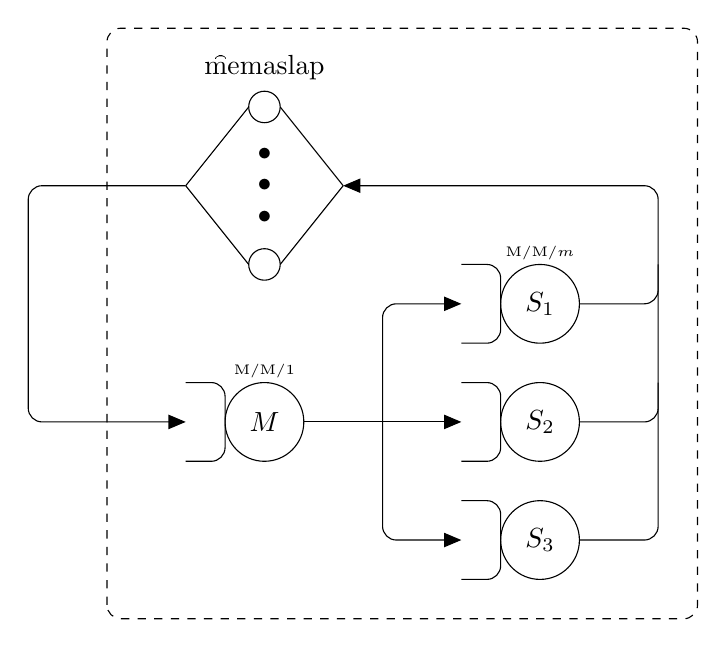
\begin{tikzpicture}[>=triangle 45]
        % Terminals.
        \draw (2,6.5) node {\t{memaslap}};
        \draw (2,6) circle (0.2);
        \draw (2,5.4) node {$\bullet$};
        \draw (2,5) node {$\bullet$};
        \draw (2,4.6) node {$\bullet$};
        \draw (2,4) circle (0.2);
        \draw (3,5) -- (2.2,6);
        \draw (3,5) -- (2.2,4);
        \draw (1,5) -- (1.8,6);
        \draw (1,5) -- (1.8,4);
        
        % Queues.
        \draw (2,2.65) node {\tiny{M/M/1}};
        \draw (2,2) circle (0.5) node {$M$};
        \draw[rounded corners=5] (1,1.5) -- (1.5,1.5) -- (1.5,2.5) -- (1,2.5);
        \draw (5.5,4.15) node {\tiny{M/M/$m$}};
        \draw (5.5,3.5) circle (0.5) node {$S_1$};
        \draw[rounded corners=5] (4.5,3) -- (5,3) -- (5,4) -- (4.5,4);
        \draw (5.5,2) circle (0.5) node {$S_2$};
        \draw[rounded corners=5] (4.5,1.5) -- (5,1.5) -- (5,2.5) -- (4.5,2.5);
        \draw (5.5,0.5) circle (0.5) node {$S_3$};
        \draw[rounded corners=5] (4.5,0) -- (5,0) -- (5,1) -- (4.5,1);
        
        % Connections.
        \draw[->] (2.5,2) -- (4.5,2);
        \draw[->,rounded corners=5] (3.5,2) -- (3.5,3.5) -- (4.5,3.5);
        \draw[->,rounded corners=5] (3.5,2) -- (3.5,0.5) -- (4.5,0.5);
        \draw[->,rounded corners=5] (6,3.5) -- (7,3.5) -- (7,5) -- (3,5);
        \draw[rounded corners=5] (6,2) -- (7,2) -- (7,4);
        \draw[rounded corners=5] (6,0.5) -- (7,0.5) -- (7,2.5);
        \draw[->,rounded corners=5] (1,5) -- (-1,5) -- (-1,2) -- (1,2);
        
        % Outer box.
        \draw[rounded corners=5,dashed] (0,-0.5) rectangle (7.5,7);
    \end{tikzpicture}
    \caption{The system modeled as a network of queues.}
    \label{fig:3_network_}
\end{figure}










\begin{figure}[!h]
\centering
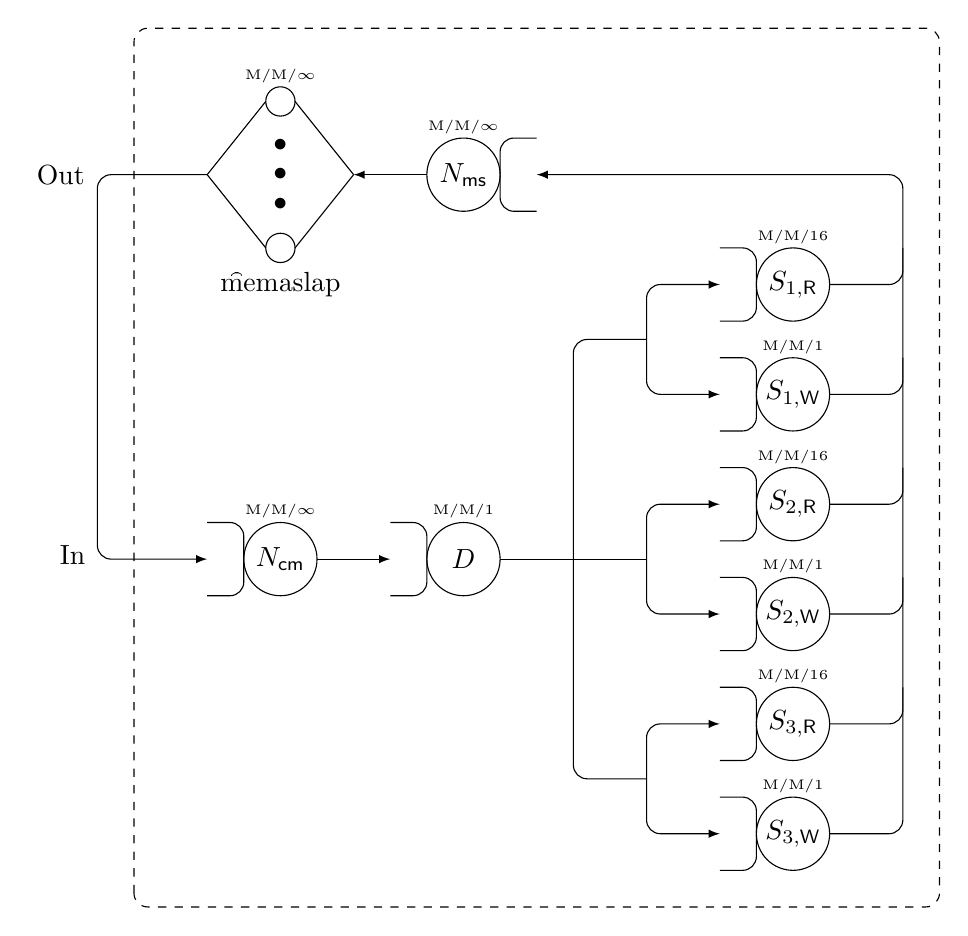
\begin{tikzpicture}[>=latex,scale=0.93]

% DEVICES

% Clients.
\draw (2,11.35) node {\tiny{M/M/$\infty$}};
\draw (2,11) circle (0.2);
\draw (2,10.4) node {$\bullet$};
\draw (2,10) node {$\bullet$};
\draw (2,9.6) node {$\bullet$};
\draw (2,9) circle (0.2);
\draw (3,10) -- (2.2,11);
\draw (3,10) -- (2.2,9);
\draw (1,10) -- (1.8,11);
\draw (1,10) -- (1.8,9);
\draw (2,8.5) node {\t{memaslap}};

% Clients-middleware connection.
\draw (2,5.4) node {\tiny{M/M/$\infty$}};
\draw (2,4.75) circle (0.5) node {$N_{\textsf{cm}}$};
\draw[rounded corners=5] (1,4.25) -- (1.5,4.25) -- (1.5,5.25) -- (1,5.25); 

% Dispatcher.
\draw (4.5,5.4) node {\tiny{M/M/$1$}};
\draw (4.5,4.75) circle (0.5) node {$D$};
\draw[rounded corners=5] (3.5,4.25) -- (4,4.25) -- (4,5.25) -- (3.5,5.25);

% Reader for server 1.
\draw (9,9.15) node {\tiny{M/M/$16$}};
\draw (9,8.5) circle (0.5) node {$S_{1,\textsf R}$};
\draw[rounded corners=5] (8,8) -- (8.5,8) -- (8.5,9) -- (8,9);

% Writer for server 1.
\draw (9,7.65) node {\tiny{M/M/$1$}};
\draw (9,7) circle (0.5) node {$S_{1,\textsf W}$};
\draw[rounded corners=5] (8,6.5) -- (8.5,6.5) -- (8.5,7.5) -- (8,7.5);

% Reader for server 2.
\draw (9,6.15) node {\tiny{M/M/$16$}};
\draw (9,5.5) circle (0.5) node {$S_{2,\textsf R}$};
\draw[rounded corners=5] (8,5) -- (8.5,5) -- (8.5,6) -- (8,6);

% Writer for server 2.
\draw (9,4.65) node {\tiny{M/M/$1$}};
\draw (9,4) circle (0.5) node {$S_{2,\textsf W}$};
\draw[rounded corners=5] (8,3.5) -- (8.5,3.5) -- (8.5,4.5) -- (8,4.5);

% Reader for server 3.
\draw (9,3.15) node {\tiny{M/M/$16$}};
\draw (9,2.5) circle (0.5) node {$S_{3,\textsf R}$};
\draw[rounded corners=5] (8,2) -- (8.5,2) -- (8.5,3) -- (8,3);

% Writer for server 3.
\draw (9,1.65) node {\tiny{M/M/$1$}};
\draw (9,1) circle (0.5) node {$S_{3,\textsf W}$};
\draw[rounded corners=5] (8,0.5) -- (8.5,0.5) -- (8.5,1.5) -- (8,1.5);

% Middleware-clients connection.
\draw (4.5,10.65) node {\tiny{M/M/$\infty$}};
\draw (4.5,10) circle (0.5) node {$N_{\textsf{ms}}$};
\draw[rounded corners=5] (5.5,9.5) -- (5,9.5) -- (5,10.5) -- (5.5,10.5);

% CONNECTIONS

% Clients -> clients-middleware connection.
\draw[->,rounded corners=5] (1,10) -- (-0.5,10) -- (-0.5,4.75) -- (1,4.75);

% Clients-middleware connection -> dispatcher.
\draw[->] (2.5,4.75) -- (3.5,4.75);

% Dispatcher -> readers/writers.
\draw (5,4.75) -- (7,4.75);
\draw[rounded corners=5] (7,1.75) -- (6,1.75) -- (6,7.75) -- (7,7.75);
\draw[<->,rounded corners=5] (8,1) -- (7,1) -- (7,2.5) -- (8,2.5);
\draw[<->,rounded corners=5] (8,4) -- (7,4) -- (7,5.5) -- (8,5.5);
\draw[<->,rounded corners=5] (8,7) -- (7,7) -- (7,8.5) -- (8,8.5);

% Readers/writers -> middleware-clients connection.
\draw[->,rounded corners=5] (9.5,8.5) -- (10.5,8.5) -- (10.5,10) -- (5.5,10);
\draw[rounded corners=5] (9.5,7) -- (10.5,7) -- (10.5,9);
\draw[rounded corners=5] (9.5,5.5) -- (10.5,5.5) -- (10.5,7.5);
\draw[rounded corners=5] (9.5,4) -- (10.5,4) -- (10.5,6);
\draw[rounded corners=5] (9.5,2.5) -- (10.5,2.5) -- (10.5,4.5);
\draw[rounded corners=5] (9.5,1) -- (10.5,1) -- (10.5,3);

% Middleware-clients connection -> clients.
\draw[->] (4,10) -- (3,10);

% OTHER

% Outer box.
\draw[rounded corners=5,dashed] (0,0) rectangle (11,12);

% In/Out labels.
\draw (-0.84,4.8) node {In};
\draw (-1,10) node {Out};

\end{tikzpicture}
\caption{The system modeled as a network of queues.}
\label{fig:3_network__}
\end{figure}












\begin{figure}[!h]
\centering
%\begin{tikzpicture}[>=latex,scale=0.99]
\begin{tikzpicture}[>=triangle 45,scale=0.99]

% DEVICES

% Clients.
\draw (2,11.85) node {\tiny{M/M/$\infty$}};
\draw (2,11.5) circle (0.2);
\draw (2,10.9) node {$\bullet$};
\draw (2,10.5) node {$\bullet$};
\draw (2,10.1) node {$\bullet$};
\draw (2,9.5) circle (0.2);
\draw (3,10.5) -- (2.2,11.5);
\draw (3,10.5) -- (2.2,9.5);
\draw (1,10.5) -- (1.8,11.5);
\draw (1,10.5) -- (1.8,9.5);
\draw (2,9) node {\t{memaslap}};

% Clients-middleware connection.
\draw (2,5.4) node {\tiny{M/M/$\infty$}};
\draw (2,4.75) circle (0.5) node {$C_{\textsf{cm}}$};
\draw[rounded corners=5] (1,4.25) -- (1.5,4.25) -- (1.5,5.25) -- (1,5.25); 

% Dispatcher.
\draw (4.5,5.4) node {\tiny{M/M/$1$}};
\draw (4.5,4.75) circle (0.5) node {$D$};
\draw[rounded corners=5] (3.5,4.25) -- (4,4.25) -- (4,5.25) -- (3.5,5.25);

% Reader 1.
\draw (9,9.65) node {\tiny{M/M/$16$}};
\draw (9,9) circle (0.5) node {$R_1$};
\draw[rounded corners=5] (8,8.5) -- (8.5,8.5) -- (8.5,9.5) -- (8,9.5);

% Writer 1.
\draw (9,8.15) node {\tiny{M/M/$1$}};
\draw (9,7.5) circle (0.5) node {$W_1$};
\draw[rounded corners=5] (8,7) -- (8.5,7) -- (8.5,8) -- (8,8);

% Reader 2.
\draw (9,6.15) node {\tiny{M/M/$16$}};
\draw (9,5.5) circle (0.5) node {$R_2$};
\draw[rounded corners=5] (8,5) -- (8.5,5) -- (8.5,6) -- (8,6);

% Writer 2.
\draw (9,4.65) node {\tiny{M/M/$1$}};
\draw (9,4) circle (0.5) node {$W_2$};
\draw[rounded corners=5] (8,3.5) -- (8.5,3.5) -- (8.5,4.5) -- (8,4.5);

% Reader 3.
\draw (9,2.65) node {\tiny{M/M/$16$}};
\draw (9,2) circle (0.5) node {$R_3$};
\draw[rounded corners=5] (8,1.5) -- (8.5,1.5) -- (8.5,2.5) -- (8,2.5);

% Writer 3.
\draw (9,1.15) node {\tiny{M/M/$1$}};
\draw (9,0.5) circle (0.5) node {$W_3$};
\draw[rounded corners=5] (8,0) -- (8.5,0) -- (8.5,1) -- (8,1);

% Server 1.
\draw (12.5,8.9) node {\tiny{M/M/$1$}};
\draw (12.5,8.25) circle (0.5) node {$S_1$};
\draw[rounded corners=5] (11.5,7.75) -- (12,7.75) -- (12,8.75) -- (11.5,8.75);

% Server 2.
\draw (12.5,5.4) node {\tiny{M/M/$1$}};
\draw (12.5,4.75) circle (0.5) node {$S_2$};
\draw[rounded corners=5] (11.5,4.25) -- (12,4.25) -- (12,5.25) -- (11.5,5.25);

% Server 3.
\draw (12.5,1.9) node {\tiny{M/M/$1$}};
\draw (12.5,1.25) circle (0.5) node {$S_3$};
\draw[rounded corners=5] (11.5,0.75) -- (12,0.75) -- (12,1.75) -- (11.5,1.75);

% Middleware-clients connection.
\draw (4.5,11.15) node {\tiny{M/M/$\infty$}};
\draw (4.5,10.5) circle (0.5) node {$C_{\textsf{ms}}$};
\draw[rounded corners=5] (5.5,10) -- (5,10) -- (5,11) -- (5.5,11);

% CONNECTIONS

% Clients -> clients-middleware connection.
\draw[->,rounded corners=5] (1,10.5) -- (-0.5,10.5) -- (-0.5,4.75) -- (1,4.75);

% Clients-middleware connection -> dispatcher.
\draw[->] (2.5,4.75) -- (3.5,4.75);

% Dispatcher -> readers/writers.
\draw (5,4.75) -- (7,4.75);
\draw[rounded corners=5] (7,1.25) -- (6,1.25) -- (6,8.25) -- (7,8.25);
\draw[<->,rounded corners=5] (8,0.5) -- (7,0.5) -- (7,2) -- (8,2);
\draw[<->,rounded corners=5] (8,4) -- (7,4) -- (7,5.5) -- (8,5.5);
\draw[<->,rounded corners=5] (8,7.5) -- (7,7.5) -- (7,9) -- (8,9);

% Readers/writers -> servers.
\draw[rounded corners=5] (9.5,9) -- (10.5,9) -- (10.5,7.5) -- (9.5,7.5);
\draw[->,rounded corners=5] (10.5,8.25) -- (11.5,8.25);
\draw[rounded corners=5] (9.5,5.5) -- (10.5,5.5) -- (10.5,4) -- (9.5,4);
\draw[->,rounded corners=5] (10.5,4.75) -- (11.5,4.75);
\draw[rounded corners=5] (9.5,2) -- (10.5,2) -- (10.5,0.5) -- (9.5,0.5);
\draw[->,rounded corners=5] (10.5,1.25) -- (11.5,1.25);

% Servers -> middleware-clients connection.
\draw[->,rounded corners=5] (13,8.25) -- (14,8.25) -- (14,10.5) -- (5.5,10.5);
\draw[rounded corners=5] (13,4.75) -- (14,4.75) -- (14,8.5);
\draw[rounded corners=5] (13,1.15) -- (14,1.15) -- (14,5);

% Middleware-clients connection -> clients.
\draw[->] (4,10.5) -- (3,10.5);

% OTHER

% Outer box.
\draw[rounded corners=5,dashed] (0,-0.5) rectangle (14.5,12.5);

% In/Out labels.
\draw (-0.84,4.8) node {In};
\draw (-1,10.5) node {Out};

\end{tikzpicture}
\caption{The system modeled as a network of queues.}
\label{fig:3_network___}
\end{figure}
\end{comment}